\title{Velocity Inversion by Surface Source Extension}
\author{William. W. Symes \thanks{The Rice Inversion Project,
Department of Computational and Applied Mathematics, Rice University,
Houston TX 77251-1892 USA, email {\tt symes@caam.rice.edu}.}}

\lefthead{Symes}

\righthead{Velocity Inversion by Surface Source Extension}

\maketitle
\begin{abstract}
Extension methods reformulate inverse problems in wave propagation by adding degrees of freedom to the domain of an objective function, the minimizer of which is the solution of the inverse problem. In favorable cases the modified objective function has a larger domain of convexity than does the original, leading to effective solution of the inverse problem via numerical optimization. Source extension adds degrees of freedom to the energy source representation. When the extended sources are confined to a hypersurface, they are uniquely determined by velocity and other material parameters, even when those parameters are inconsistent with the data of the in verse problem. This ability of extended surface sources to fit data regardless of the choice of other parameters is one of the crucial links in the relation of a natural extended objective function with travel time tomography.


\end{abstract}

\inputdir{../trans/project}

\section{Full Waveform Inversion}

A simple example: acoustic transmission inversion - isotropic point radiator (``source'') located at  $\bx=\bx_s$
\begin{equation}
\label{eqn:awept}
\frac{1}{\kappa}\frac{\partial p}{\partial t} = -\nabla \cdot {\bf v} + f(t)\delta(\bx-\bx_s), \,\rho \frac{\partial {\bf v}}{\partial t} = - \nabla p; \,p,{\bf v}=0, t \ll 0
\end{equation}
Bulk modulus is depicted in Figure \ref{fig:bml0}.

\plot{bml0}{width=\textwidth}{Lens example: target bulk modulus $\kappa$}

$x_s=3500$ m, $z_s=3000$ m, receiver positions $x_r=2000-6000$ m, $z_r=1000$ m



Modeling operator $(S[\kappa]f)(t,x_r) = \phi(x_r) p(t,x_r,z_r)$ - linear in $f$, nonlinear in $\kappa$

%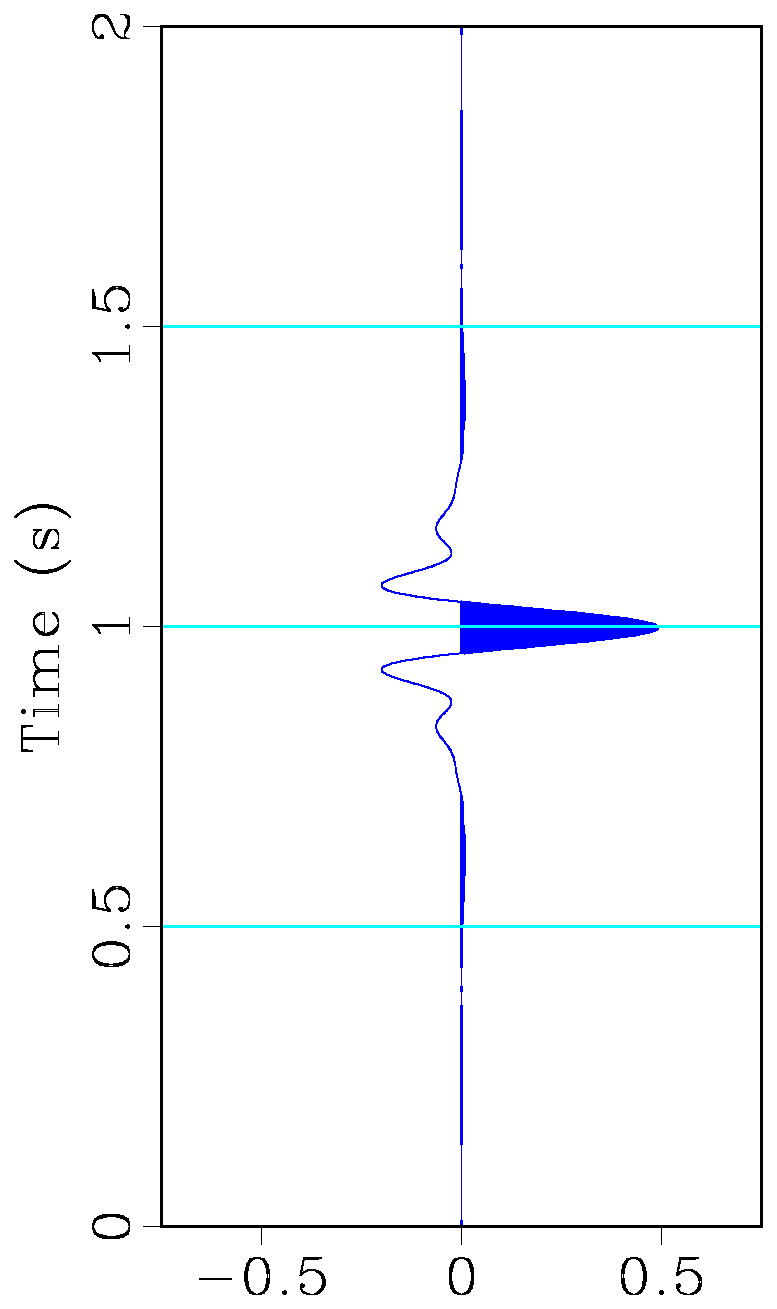
\includegraphics[height=1.5in]{Fig/pulse00.pdf} %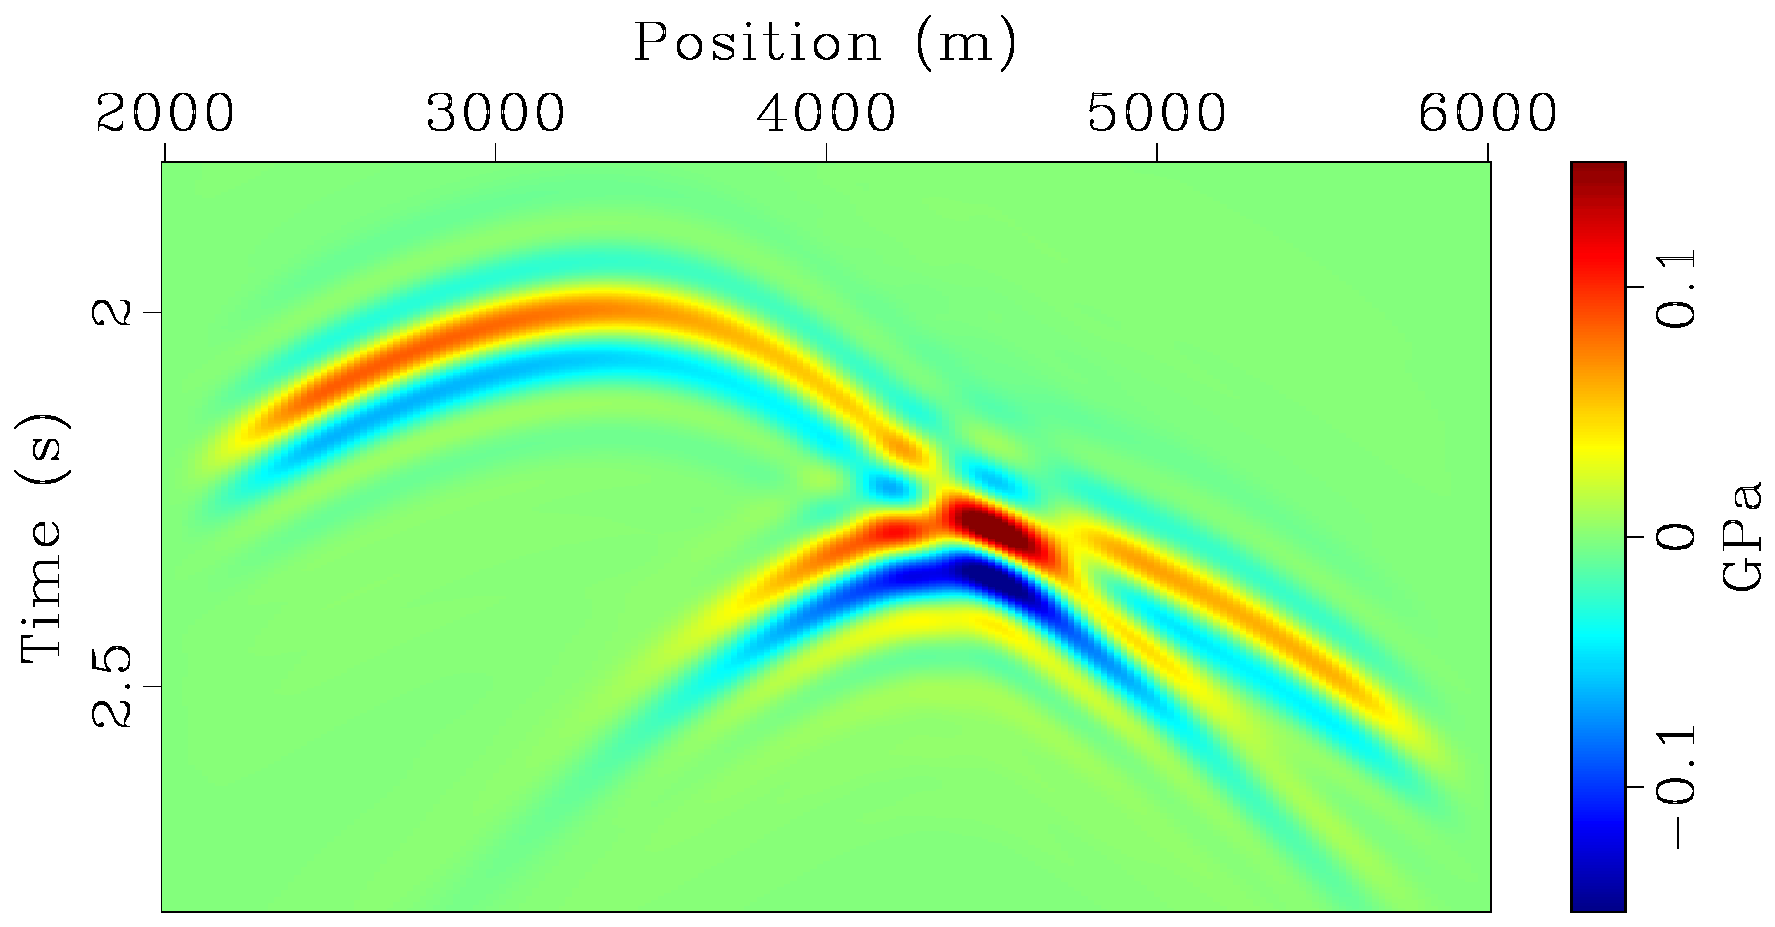
\includegraphics[height=1.5in]{Fig/ptpwindl0.pdf}\\
\plot{pulse00}{width=0.5\textwidth}{Bandpass filter pulse $f$}
\plot{ptpwindl0}{width=\textwidth}{Receiver line  $S(\kappa)$  at $z_r=1$ km for source at $z_s=3$ km, $x_s=3$ km. bulk modulus $\kappa$ with low velocity lens as in Figure \ref{fig:bml0}, $\rho$=1 g/cm$^{3}$. Coarse grid: $dx=dz=20$ m, $dt=$ 8 ms, (2,4) staggered grid scheme. }
% at receiver position $1000 m$ for source at $x=3500$ m, $z=3000$ m}

{\bf F}ull {\bf W}aveform {\bf I}nversion = output least squares: minimize over $\kappa$ (for example)
\[
J_{\rm FWI}[\kappa,d] = \frac{1}{2}\|S[\kappa]f-d\|^2
\]
Variants of Newton's method use preconditioned gradient
\[
\nabla J_{\rm FWI}[\kappa,d] = W^{-1}DS[\kappa]^T(S[\kappa]f-d)
\]
$W^{-1}$ = preconditioner $\Leftrightarrow$ $W$ = Gram op for inner product on model space

{\color{blue} this talk: constrain bulk modulus $\kappa$ to be {\em smooth} ($\Rightarrow W^{-1}$ smoothing), density $\rho$ constant \& fixed}

What goes wrong: ``cycle skipping'', ``trapped in local minima'',...

Assume local geometric optics: $\tau(x_s,x_r) =$ ray travel time from $(x_s,z_s)$ to $(x_r,z_r)$, $a(x_s,x_r)$ = geometric amplitude
\[
S[\kappa]f(\bx_r,t) \approx a(x_s,x_r)f(t-\tau(x_s,x_r))
\]
then $S[\kappa]f=d$ $\Rightarrow$
\[
D^2J_{\rm FWI}[\kappa,d](\delta \kappa,\delta \kappa) \approx \|(...)D\tau[\kappa]\delta \kappa\|^2\left\|\frac{df}{dt}\right\|^2
\]
High frequency asymptotics: $f_{\lambda}(t) = \frac{1}{\sqrt{\lambda}} f\left(\frac{t}{\lambda}\right), d_{\lambda} = S[\kappa]f_{\lambda}$ 

$
\|D\tau[\kappa]\delta \kappa\|=O(1) \Rightarrow D^2J_{\rm FWI}[\kappa,d_{\lambda}](\delta \kappa,\delta \kappa)=O(\lambda^{-2})$ but $ J_{\rm FWI}[\kappa,d_{\lambda}]=O(1)
$
$\Rightarrow$ {\color{blue} $J_{\rm FWI}$ convex in region of diameter $O(\lambda)$}

Extension of $S$ = map $\oS$ on larger domain, with embedding $E$ 
\[
S = \oS \circ E
\]
Annihilator $A$: $\mbox{ker }A = \mbox{range E}$. 

Example - {\bf S}urface {\bf S}ource {\bf E}xtension 

Domain of $\oS = \{\mbox{(smooth bulk moduli)} \times {\cal E}'\{z=z_s, x_s-r < x < x_s+r\} \}$

Compute $\oS$: solve wave equation with point source {\color{blue} $f(t)\delta(x-x_s)$}$\delta(z-z_s)$ replaced by {\color{blue}$\of(t,x)$}$\delta(z-z_s) \in {\cal E}\{z=z_s, x_s-r < x < x_s+r\}$

\begin{equation}
\label{eqn:extann}
Ef(t,x) = f(t)\delta(x-x_s),\,A\of(t,x)=(x-x_s)\of(t,x)
\end{equation}

Big deal: $\oS[\kappa]$ has a microlocal approximate inverse $\oS[\kappa]^{\dagger}$ [$S$ has approximate left inverse {\em but not right!}]:
\begin{eqnarray}
\oS[\kappa]^{\dagger}\oS[\kappa] &=& \Pi_s[\kappa]\\
\oS[\kappa]\oS[\kappa]^{\dagger} &=& \Pi_r[\kappa]
\end{eqnarray}
The approximate projectors $\Pi_s,\Pi_r \in OPS^0$ have symbols $\equiv 1$ in conic $\gamma_{s,r} \subset T^*(\Gamma_{s,r})$

%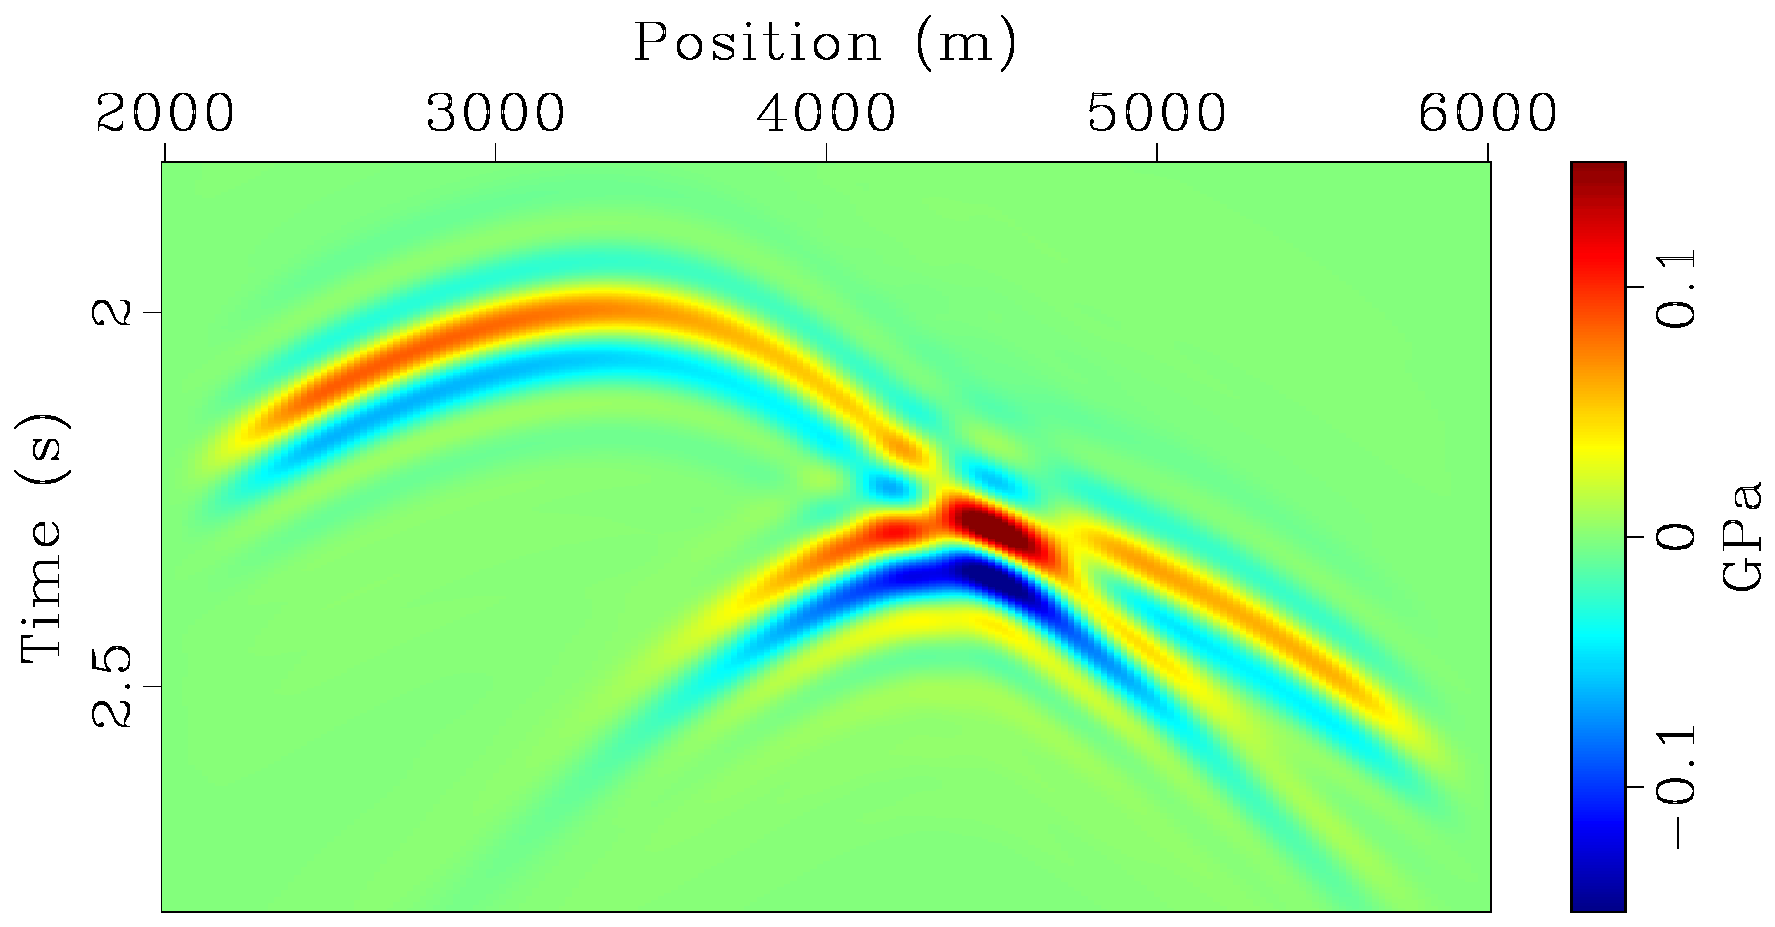
\includegraphics[height=1.2in]{Fig/ptpwindl0.pdf}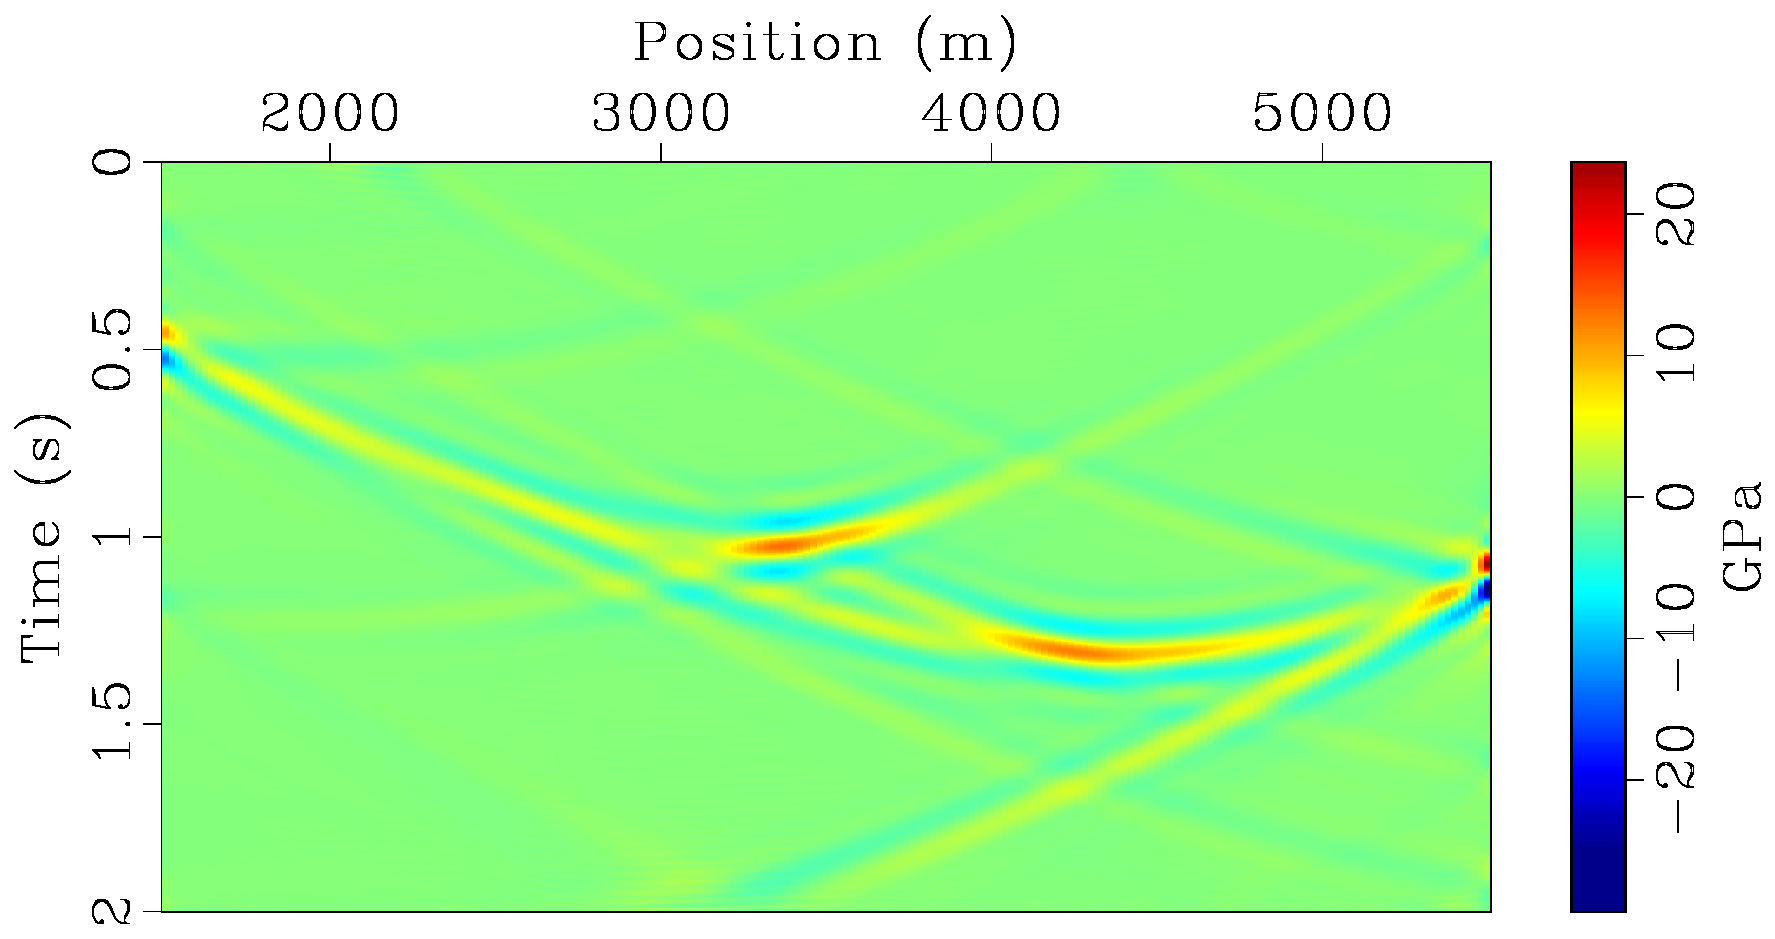
\includegraphics[height=1.2in]{Fig/cgwhestsourceplh0.pdf}\\
\plot{cgwhestsourceplh0}{width=\textwidth}{$\of=\oS(\kappa_0)^{\dagger}d$ for $\kappa_0 \equiv 4.0$ GPa, approx. via CG - $r=2000 m$}

At solution source should be supported at $x=x_s$ - in $\mbox{rng }E = \mbox{ker }A$

One way to incorporate this: penalty function
\begin{equation}
\label{eqn:Jnaive}
\tilde{J}_{\alpha}[\kappa,\of,d] = \frac{1}{2}(\|\oS[\kappa]\of -d\|^2 + \alpha^2 \|A\of\|^2)
\end{equation}

Reduced objective:
\[
J_{\alpha}[\kappa,d] = \mbox{min}_{\of} \tilde{J}_{\alpha}[\kappa,\of,d] = \tilde{J}_{\alpha}[\kappa,\of_{\alpha}[\kappa,d],d]
\]
$\of_{\alpha}[\kappa,d]$ = solution of {\em inner problem}
\[
N_{\alpha}[\kappa]\of = \oS[\kappa]^Td,\,\,N_{\alpha}[\kappa] = \oS[\kappa]^T\oS[\kappa] + \alpha^2 A^TA
\]

Solving the outer problem (``variable projection method'', Golub \& Pereyra 73, 03):
\[
\nabla J_{\alpha}[\kappa,d] = W^{-1} D\oS[\kappa]^T(\of_{\alpha}[\kappa,d],\oS[\kappa]\of_{\alpha}[\kappa,d]-d)
\]
closely resembles FWI gradient, efficiently computable via adjoint state method

Algorithm:
\begin{itemize}
\item solve inner problem using CG
\item adjust $\alpha$ using Discrepancy Principle (keep residual $\in (e_-, e_+)$) - $\oS^{\dagger} \Rightarrow$ can start with $\alpha=0$ (Fu \& S. 17)
\item outer update using steepest descent, line search
\end{itemize}



\section{Modeling}

First, a formal definition of $\oS$: choose cutoff functions $\chi_a \in C_0^{\infty}(\Gamma_a \times \bR)$ with $a \in \{s,r\}$. For $\of \in C_0^{\infty}(\Gamma_s \times \bR)$, the initial value problem
\begin{equation}
\label{eqn:awept}
\frac{1}{\kappa}\frac{\partial p}{\partial t} = -\nabla \cdot {\bf v} + \chi_s\of, \,\rho \frac{\partial {\bf v}}{\partial t} = - \nabla p; \,p,{\bf v}=0, t \ll 0
\end{equation}
has a unique solution $(p,\bv)$, smooth except on $\Gamma_s \times \bR$. 
Define
\begin{equation}
\label{eqn:os1def}
\oS_1[\kappa]\of = \chi_r p|_{\Gamma_r \times \bR}
\end{equation}

First Key Observation: adopt

\noindent {\bf Assumption A:} There exists $\theta_*>0$ so that for every ray connecting a point in $\mbox{supp }\chi_s$ with a point in $\mbox{supp }\chi_r$, the angles $\theta_s$ and $\theta_r$ subtended by the ray and the tangent planes of $\Gamma_s$ and $\Gamma_r$ respectively are both greater than $\theta_*$ in absolute value.

Denote by $\gamma_{s,r}$ the open set of rays $\{(\bx,r \xi): r>0\}$ through projections $(\bx,\xi)$ onto $T^*(\Gamma_{s,r} \times \bR)$ of initial/final conditions for rays connecting points in the interiors of $\mbox{supp }\chi_{s,r}$: these are open conic sets. Note that $\gamma_{s,r}$ is $\kappa$-dependent. If $C[\kappa]$ denotes the twisted canonical relation for $\oS$, $\gamma_r = C[\kappa]\gamma_s$.

Then 
$\oS_1[\kappa]$ has a microlocal approximate inverse $(\oS[\kappa]^1)^{\dagger}$, defined by 
\begin{equation}
\label{eqn:appinv}
\oS_1^{\dagger} = W_s^{-1}\oS_1^TW_r
\end{equation}
in which $W_s, W_r$ are properly supported $\Psi$DOs on $\Gamma_s \times \bR,\Gamma_r \times \bR$ respectively [from here on, suppress the arguments whenever these are obvious: $\oS_1 = \oS_1[\kappa]$ and so on]. The sense in which $\oS_1^{\dagger}$ is an inverse is that
\begin{eqnarray}
\label{eqn:proj}
\oS_1^{\dagger}\oS &=& \Pi^1_s\\
\oS \oS_1^{\dagger} &=& \Pi^1_r
\end{eqnarray}
in which $\Pi^1_{s,r} \in OPS^0(\Gamma_{s,r}\times \bR)$ have principal symbols $\sim 1$ in the conic sets $\gamma_{s,r} \subset T^*(\Gamma_{s,r}\times \bR)$.
%, and $\ge 1/2$ in the larger conic sets $\tilde{\gamma}^1_{s,r} \supset \gamma^1_{s,r}$.

It follows immediately from \ref{eqn:proj} that
\begin{equation}
\label{eqn:picomm}
\oS_1 \Pi^1_s = \Pi^1_r\oS_1
\end{equation}

The (G\^{a}teaux) derivative $D\oS_1 = D\oS_1[\kappa]\delta \kappa$ (that is, a perturbation $\delta \kappa \in C_0^{\infty}(\bR^d)$ is implicit in the notation) is a Fourier Integral Operator operator of order 1, with the same canonical relation: a proof of this statement is given in appendix 1. It follows that
\begin{eqnarray}
\label{eqn:qdef}
Q_s &\equiv& \oS_1^{\dagger}D\oS_1 \nonumber \\
Q_r &\equiv& D\oS_1 \oS_1^{\dagger} 
\end{eqnarray}
are microlocally eilliptic $\Psi$DOs of order 1, and satisfy
\begin{eqnarray}
\label{eqn:qrel}
\oS_1 Q_s &=& \Pi^1_r D\oS_1 \nonumber \\
Q_r \oS_1 &=& D\oS_1 \Pi^1_s \nonumber \\
Q_s\oS_1^{\dagger} &=& \oS_1^{\dagger} Q_r
\end{eqnarray}
Since $D\oS_1$ is linear in $\delta \kappa$, so is $Q_{s,r} = Q_{s,r}[\kappa]\delta \kappa$.

\begin{lemma}\label{thm:qskew} $Q_s$ is essentially skew-symmetric, that is, $B \equiv Q_s+Q_s^T \in OPS^0(\Gamma_s \times \bR)$.
\end{lemma}

\begin{proof}: In the definition $\oS_1^{\dagger}=W_s^{-1}\oS_1^TW_r$, the weights $W_s, W_r$ are symmetric invertible members of $OPS^{0}(\Gamma_{s,r} \times \bR)$.
\[
D(\oS_1^{\dagger}\oS_1) = D\Pi^1_s
\]
\[
=D(W_m^{-1})\oS_1^TW_d \oS_1 + W_m^{-1}D\oS_1^TW_d \oS_1 + W_m^{-1}\oS_1^TDW_d \oS_1 + W_m^{-1}\oS_1^TW_dD\oS_1
\]
Also 
\[
Q_s^T = D\oS_1^T W_d ^T\oS_1 W_m^{-1}
\]
so
\[
W_m^{-1}Q_s^TW_m = W_m^{-1}D\oS_1^TW_d \oS_1
\]
is identical to the second term above, and by the $\Psi$DO calculus differs from $Q_s^T$ by a member of  $OPS^0(\Gamma_S \times \bR)$. The first and the third define members of $OPS^0(\Gamma_S \times \bR)$, by the rules for composition of FIO, and the fourth term is $Q_s$. \end{proof}

Select $\kappa^0 \in C^{\infty}(\bR^d)$, and choose a neighborhood $U \subset C^{\infty}(\bR^d)$ of $\kappa_0$ so that there exist non-void open conic subsets $\gamma^0_s, \tilde{\gamma}^0_s$ of $ T^*(\Gamma_{s,r} \times \bR)$ with $\overline{\tilde{\gamma}^0_s} \subset \gamma^0_s$ so that for $\kappa \in U$, 
\begin{itemize}
\item[A1: ] $\gamma^0_s \subset \gamma_s[\kappa]$
\item[A2: ] $C[\kappa]\gamma^0_s \subset  \gamma_r[\kappa]$
\end{itemize}
(recall that $C[\kappa]$ is the twisted canonical relation of $S$).

Let $\Pi_s$ denote an order zero $\Psi$DO with principal symbol $\sim 1$ in $\tilde{\gamma}^0_s$, $\mbox{ess supp }\Pi_s \subset \gamma^0_s$. From relation \ref{eqn:picomm}
\begin{eqnarray}
\label{eqn:pistuff3}
\Pi^1_r \oS_1 \Pi_s = \oS_1 \Pi^1_s \Pi_s  =\oS_1(\Pi_s^1-I)\Pi_s + \oS_1 \Pi_s
\end{eqnarray}
Since the symbol of $\Pi^1_s$ is $ \sim 1$ on $\mbox{ess supp}(\Pi_s)$, $(\Pi_s^1-I)\Pi_s \in OPS^{-\infty}(\Gamma_s \times \bR)$. Thus the first term on the RHS in equation aboveis (infinitely) smoothing, 

In the sequel, I will write $\approx$ for ``differs by smoothing operator''. Thus
\begin{eqnarray}
\label{eqn:pistuff3}
\Pi^1_r \oS_1 \Pi_s \approx \oS_1 \Pi_s
\end{eqnarray}
Define 
\begin{equation}
\label{osdef}
\oS = \oS_1 \Pi_s
\end{equation}
Since $\Pi_s$ is independent of $\kappa \in U$,
\[
D\oS = D\oS_1 \Pi_s \approx (\Pi^1_r D\oS_1-D\Pi \oS_1 \Pi_s)
\]
from \ref{eqn:pistuff3}. The second term on the RHS is smoothing because of the null intersection of essential supports, so
\[
\approx \oS_1 Q_s \Pi_s = \oS Q_s + \oS_1 [Q_s,\Pi_s]+ = \oS(Q_s+[Q_s,\Pi_s]) + \oS_1(I-\Pi_s)[Q_s,\Pi_s]
\]
Thus
\begin{equation}
\label{eqn:qrel0}
D\oS \approx \oS Q + \oS_1R
\end{equation}
in which $Q=Q_s + [Q_s,\Pi_s] \in OPS^1(\Gamma_s \times \bR)$ and $R = (I-\Pi_s)[Q_s,\Pi_s] \in OPS^0(\Gamma_s \times \bR)$. Note that the principal symbols of $Q$ and $Q_s$ are identical, and 
\begin{equation}
\label{eqn:esssuppr}
\mbox{ess supp}(R) \subset \gamma_s \setminus \tilde{\gamma}_s.
\end{equation}
That is, $R$ is essentially supported near the boundary of $\gamma_s$.

\section{Regularization}
The naive version of the least squares problem given in definition \ref{eqn:Jnaive} is unsatisfactory for several reasons. First, the intended null space of the annihilator (equation \ref{eqn:extann}) does not lie in its domain ($L^2$): in fact, the null space is actually the $\{0\}$. Moreover, the multiplier defining $A$ has a singularity, so $A$ is not pseudodifferential. Second, the normal operator of the least squares problem of minimizing the function \ref{eqn:Jnaive} is not coercive, so there is no guarantee that the reduced form is well-defined. Therefore the variable projection method actually makes no sense for this problem.

Two amendments remedy both problems. To give the annihilator a nonempty null space approximating the desired one (i.e. supported near $\bx_s$), and make it a pseudodifferential operator, cut it off smoothly near $\bx_s$. Specifically, choose $\chi_1 \in C_0^{\infty}(\bR^d)$ so that $\chi_1(x)=0$ for $|x|<1$, $\chi_1(x)=1$ for $|x| >2$. For $r>0$, define $\chi_r \in C_0^{\infty}(\bR^d)$ by
\[
\chi_r(x) = \chi_1(x/r).
\]
Then set 
\[
A_r = A(1-\chi_{2r}), \, Au(\bx,t)=|\bx-\bx_s|u(\bx,t)|
\]
$A_r$ is a regularized version of $A$, the null space of which consists of square-integrable functions supported in the cylinder $|\bx-\bx_s| \le r$. In practice, $r$ might be chosen to be a couple of wavelengths (or even ignored altogether - this seems to work, though it is not altogether clear why). Since the multiplier defining $A_r$ is smooth, $A_r$ is also pseudodifferential of order $0$.

The second problem is solved simply by Tihonov regularization. Introduce an additional penalty proportional to $\|\of\|^2$:
\begin{equation}
\label{eqn:jdef}
\Ja[\kappa,\of]=\frac{1}{2}(\|\oS \of - d\|^2 + \alpha^2 \|A_r\of\|^2 + \lambda^2\|\of\|^2)
\end{equation}
The normal operator 
\begin{equation}
\label{eqn:normop}
\oNa = \oS^T\oS + \alpha^2 A_r^TA_r + \lambda^2 I
\end{equation}
is coercive for $\lambda>0$, so the minimizer $\ofa=\ofa[\kappa,d]$ of $\Ja[\kappa,\cdot]$ is well-defined as the unique solution of the normal equation
\begin{equation}
\label{eqn:normal}
\oNa \ofa = \oS^Td.
\end{equation}
The reduced objective
\begin{equation}
\label{eqn:normred}
\Jared[\kappa,d] = \Ja[\kappa,\ofa[\kappa,d],d]
\end{equation}
is well-defined and smooth in its arguments.

The parametrices introduced above for $\oS_1$ lead to a useful approximation of $\ofa$. To simplify notation in the following calculations, define 
\[
M_1=\oS_1^T\oS_1,\, M=\oS^T\oS = \Pi_s^TM_1\Pi_s
\]
and
\[
M_1^{\dagger} = \oS_1^{\dagger}(\oS_1^{\dagger})^T
\]
From the definitions \ref{eqn:proj} and the relation \ref{eqn:picomm},
\[
M_1^{\dagger}M_1=\oS_1^{\dagger}(\oS_1^{\dagger})^T \oS_1^T\oS_1
=\oS_1^{\dagger}(\oS^1\oS_1^{\dagger})^T\oS_1
\]
\[
=\oS_1^{\dagger}\Pi^1_r\oS_1=\oS_1^{\dagger}\oS_1\Pi^1_s = (\Pi^1_s)^2
\]
and
\[
M_1 M_1^{\dagger}=\oS_1^T\oS_1 \oS_1^{\dagger}(\oS_1^{\dagger})^T 
=\oS_1^T(\Pi^1_r)^T(\oS_1^{\dagger})^T 
\]
\[
=(\oS_1^{\dagger}\Pi^1_r\oS_1)^T = ((\Pi^1_s)^2)^T \approx (\Pi^1_s)^2
\]
where the final equality modulo smoothing error follows from the observation the $\Pi_s$ is a scalar $\Psi$DO with real symbol, so that $\Pi_s$ and $\Pi_s^T$ have the same principal symbol.
  
That is, $M_1^{\dagger}$ is a two-sided microlocal parametrix for $M_1$. It turns out to be a parametrix for $M$ as well:
\[
M_1^{\dagger} M = M_1^{\dagger} \Pi_s M_1 \Pi_s =  M_1^{\dagger}M_1\Pi_s^2 +  M_1^{\dagger}[\Pi_s,M_1]\Pi_s
\]
The last term is in $OPS^{-1}$, so this is
\[
\approx (\Pi^1_s)^2\Pi_s^2 \approx \Pi_s^2
\]
since $\Pi^1_s\Pi_s \approx \Pi_s$ etc. Similarly,
\[
M M_1^{\dagger} \approx \Pi_s^2.
\]
That is, $M_1^{\dagger}$ is also a two-sided microlocal parametrix for $M$.

To understand the behaviour of $\ofa$ as $\lambda \rightarrow 0$ it is also useful to introduce an approximate inverse for $\oS^T\oS + \lambda^2 I = \Ml$. Define
\[
\Mld = M_1^{\dagger} (I + \lambda^2 M_1^{\dagger})^{-1}.
\]
The inverse is well-defined for $\lambda$ sufficiently small. Then
\[
(\Ml ) \Mld \approx (\Pi_s^2 + \lambda^2 M_1^{\dagger}) (I + \lambda^2 M_1^{\dagger})^{-1}
\]
\[
=I - (I-(\Pi_s)^2) (I + \lambda^2 M_1^{\dagger})^{-1}
\]
Similarly,
\[
\Mld (\Ml) \approx I - (I + \lambda^2 M_1^{\dagger})^{-1} (I-(\Pi_s)^2) 
\]
Thus $\Mld$ is a two-sided parametrix for $\Ml$ in the sense that 
\[
\Mld (\Ml) P \approx P, \, (\Ml) \Mld P \approx P
\]
for and $P \in OPS^0$ essentially supported in $\tilde{\gamma}_s$.

\section{Consistency}

I will call the triple $(\kappa,\of,d)$ {\em consistent} if $\oS[\kappa]\of = d$. A distributed source $\of\in {\cal D}(\Gamma_s \times \bR)$ is {\em $r$-approximately point} ($r>0$) if 
\begin{equation}
\label{eqn:apt}
\of = \tilde{P} f \delta_{\Gamma \times \bR},
\end{equation}
for $f \in C^{\infty}_0(\Gamma_s \times \bR)$, $\mbox{supp }f \subset B_r(\bx_s) \times \bR$ and $\tilde{P} \in OPS^0(\Gamma \times \bR)$ with essential support $\subset \tilde{\gamma}_s$. 

Will call $f$ in \ref{eqn:apt} the {\em wavelet}, and $\tilde{P}$ the {\em aperture operator}. Note that if $\of$ is $r$-approximately point, then its wavelet satisfies $f=\chi_r f$. 

\begin{lemma}
\label{thm:asm}
Suppose that $\of = \tilde{P}f$ is $r$-approximately point. Then for any $s \in \bR, B \in OPS^s(\Gamma_s \times \bR)$, 
\[
A B \of = E f
\]
in which $E \in OPS^{-\infty}(\Gamma_s \times \bR)$.
\end{lemma}
\begin{proof}
True because of pseudolocality and the null intersection of the supports of $A_r=A(1-\chi_{2r})$ and $\chi_r$.
\end{proof}

Suppose that $\of$ is approximately point, with wavelet $f$ and aperture operator $\tilde{P}$. Then
\[
(\Ml + \alpha^2 A_r^TA_r)(\ofa - \Mld M\tilde{P}f) = M\tilde{P}f 
\]
\[
- (I + (I + \lambda^2 M_1^{\dagger})^{-1} (I-(\Pi_s)^2)) M\tilde{P}\chi_rf -\alpha^2 A_r^TA_r \Mld M\tilde{P}\chi_rf
\]
\begin{equation}
\label{eqn:old}
= E f
\end{equation}
in which 
\[
E = (I + \lambda^2 M_1^{\dagger})^{-1} (I-(\Pi_s)^2) M\tilde{P} - 
-\alpha^2 A_r^TA_r \Mld M\tilde{P}\chi_r
\]
is a smoothing operator: the first term on the right is smoothing because the essential supports of $\tilde{P}$ and $(I-(\Pi_s)^2)$ have null intersection, and the second term is smoothing per Lemma \ref{thm:asm}.

I shall use $E$ as a symbol denoting various smoothing operators that occur in the calculations to come.

Now introduce a family $\{f_{\lambda}: \lambda>0\}$ of wavelets satisfying
\begin{itemize}
\item $\|f_{\lambda}\|=1$ for all $\lambda$;
\item for all $k \ge 0$, there is $c_k>0$ so that $\|(I - \Delta)^{-k/2}f_{\lambda}\| \le c_k \lambda^{-2k}$
\end{itemize}
In the last condition, $\Delta$ is the Laplace-Beltrami operator in the induced metric on $\Gamma_s \times \bR$. The condition can be interpreted as stating that $f_{\lambda}$ oscillates with wavelength $\lambda^2$. Accordingly I will call such a family {\em high-frequency}.

\begin{lemma}\label{thm:ofaerr}
Suppose that $\of$ is approximately point, with wavelet $f$ and aperture operator $\tilde{P}$, and $d=S\tilde{P}$. Then
for $s, k \ge 0$, there exist $c_{s,k}\ge 0$ so that
\begin{equation}
\label{eqn:ofaerr}
\|\ofa - \Mld M\tilde{P}f_{\lambda}\|_s \le c_{s,k}\lambda^{2k}, \,k\ge s+1
\end{equation}
\end{lemma}
\begin{proof}
\[
(\Ml + \alpha^2 A_r^TA_r)(\ofa - \Mld M\tilde{P}f) = M\tilde{P}f 
\]
\[
- (I + (I + \lambda^2 M_1^{\dagger})^{-1} (I-(\Pi_s)^2)) M\tilde{P}\chi_rf -\alpha^2 A_r^TA_r \Mld M\tilde{P}\chi_rf
\]
\begin{equation}
\label{eqn:old}
= E f
\end{equation}
in which 
\[
E = (I + \lambda^2 M_1^{\dagger})^{-1} (I-(\Pi_s)^2) M\tilde{P} - 
-\alpha^2 A_r^TA_r \Mld M\tilde{P}\chi_r
\]
is a smoothing operator: the first term on the right is smoothing because the essential supports of $\tilde{P}$ and $(I-(\Pi_s)^2)$ have null intersection, and the second term is smoothing per Lemma \ref{thm:asm}. Note that 
\[
\Ml + \alpha^2 A_r^TA_r \ge \lambda^2 I
\]
whence invertible, thanks to Lax-Milgram, with inverse bounded by $\lambda^{-2}$. So invoking the defining properties of $f_{\lambda}$,
\[
\|\ofa - \Mld M\tilde{P}f\| \le \lambda^{-2}\|Ef\| = \lambda^{-2}\|E(I-\Delta)^{k/2}(I-\Delta)^{-k/2}f_{\lambda}\|
\]
$E(I-\Delta)^{k/2}$ is smoothing hence bounded, so the second defining property of $f_{\lambda}$ gives 
\[
\le c_{0,k}\|f_{\lambda}\|\lambda^{2(k-1)}
\]
which is the $s=0$ case of the bound \ref{eqn:ofaerr}.

Assume that the bound has been established for $s-1$. Note that
\[
(I-\Delta)^{s/2}(\Ml + \alpha^2 A_r^TA_r)(\ofa - \Mld M\tilde{P}f) 
\]
\[
=(\Ml + \alpha^2 A_r^TA_r)(I-\Delta)^{s/2}(\ofa - \Mld M\tilde{P}f) 
+[(I-\Delta)^{s/2},(\Ml + \alpha^2 A_r^TA_r)](\ofa - \Mld M\tilde{P}f) 
\]
\[
=(I-\Delta)^{s/2}Ef
\]
The operator in the second term is of order $s-1$, so that contribution is bounded in $L^2$ by 
\[
\mbox{const. } \times \|\ofa - \Mld M\tilde{P}f_{\lambda}\|_{s-1} \le c_{s-1,k} \lambda^{k}
\]
for $k \ge 1$. Repeating the manipulations of the $k=0$ case, arrive at the conclusion.
\end{proof},

The next observations will permit $r$ approximately point wavelets to be treated as if they generated point sources in the null space of the penalty operator $A_r$.
\begin{lemma}
\label{thm:aptsm}
Suppose that $\{f_{\lambda}\}$ is an $r$-approximate point high frequency wavelet family, and $B \in OPS^{s}(\Gamma \times \bR)$. Then for any $s \in \bR$, $k \in {\bf N}$
\[
\|AB f_{\lambda}\|_s = O(\lambda^{2k}).
\]
\end{lemma}
\begin{proof}
Follows from Lemma \ref{thm:asm} and the defining properties of high-frequency wavelet families.
\end{proof}

\begin{lemma}
\label{thm:ofasm}
Suppose that $d=S\tilde{\Pi}f_{\lambda}$ is $r$-approximately point and $\{f_{\lambda}\}$ is a high-frequency wavelet family. Then for any $s \in \bR$, $k \in {\bf N}$, there is $C>0$ so that for sufficiently small $\lambda>0$,
\[
\|A_r \ofa\|_s \le C\lambda^{2k}
\]
\end{lemma}
\begin{proof}
From the bound \ref{eqn:ofaerr}, Lemma \ref{thm:aptsm} and the definitions above,
\[
\|A_r \ofa \|_s \le \|A_r(\ofa - \Mld M\tilde{P}f_{\lambda})\|_s + \|A_r \Mld M \tilde{P}f_{\lambda}\|_s \le c_{s,k}\lambda^{2k}
\]
for suitable $c_{s,k}>0$.
\end{proof}

\begin{lemma}
\label{thm:dataerr}
Under the assumptions of Lemma \ref{thm:ofaerr}, in particular $d_{\lambda} = \oS\tilde{P}f_{\lambda}$, for all sufficiently small $\lambda$, any $s \in \bR$, there exists $C_s>0$ so that,
\[
\|\oS \ofa - d_{\lambda}\|_s \le C_s \lambda^2.
\]
\end{lemma}
\begin{proof}
\[
\oS\ofa - d_{\lambda} = \oS(\ofa - \tilde{P}f_{\lambda}) 
\]
\begin{equation}
\label{eqn:derr1}
= \oS(\ofa - \Mld M\tilde{P}f) + \oS((\Mld M-I)\tilde{P}f)
\end{equation}
\[
\Mld M = \Mld(\Ml) - \lambda^2 \Mld \approx I - (I+\lambda^2M_1^{\dagger})^{-1}(I-\Pi_s^2) - \lambda^2 M_1^{\dagger}(I+\lambda^2M_1^{\dagger})^{-1}
\]
\[
= I - (I+\lambda^2M_1^{\dagger})^{-1}(I-\Pi_s^2) - (I+\lambda^2 M_1^{\dagger})(I+\lambda^2M_1^{\dagger})^{-1} + (I+\lambda^2M_1^{\dagger})^{-1}
\]
\[
-(I+\lambda^2M_1^{\dagger})^{-1}(I-\Pi_s^2)+ (I+\lambda^2M_1^{\dagger})^{-1}
\]
\[
= (I+\lambda^2M_1^{\dagger})^{-1}\Pi_s^2
\]
So
\[
\Mld M - I =(I+\lambda^2M_1^{\dagger})^{-1}\Pi_s^2 - (I+\lambda^2M_1^{\dagger})^{-1}(I+\lambda^2M_1^{\dagger})
\]
\[
=
(I+\lambda^2M_1^{\dagger})^{-1}(\Pi_s^2-I -\lambda^2M_1^{\dagger})
\]
whence there exists $C>0$ so that for any $k>0$, sufficiently small $\lambda$,
\[
\|\oS\ofa - d\|_s  \le C (\|\ofa - \Mld M\tilde{P}f_{\lambda}\|_s 
\]
\[
+ \|(I+\lambda^2M_1^{\dagger})^{-1}(\Pi_s^2-I -\lambda^2M_1^{\dagger})\tilde{P}f_{\lambda}\|_s
\]
\[
\le C(\lambda^{2k} + \lambda^2\|(I+\lambda^2M_1^{\dagger})^{-1}M_1^{\dagger}\tilde{P}f_{\lambda}\|_s)
\]
\[
\le C_s\lambda^2
\]
for suitable choice of $C_s > 0$.
\end{proof}


\section{Derivatives}
The variable projection method amounts to minimization of the reduced objective
\[
\Jared[\kappa] = \Ja[\kappa,\ofa[\kappa]].
\]
It follows from the normal equation \ref{eqn:normal} that the derivative of $\Jared$ is given by
VPM derivative formula:
\[
D\Jared[\kappa]\delta \kappa = \langle D(\oS[\kappa] \ofa[\kappa])\delta[\kappa],\oS[\kappa] \ofa[\kappa] -d\rangle
\]
To simplify notation, in the following I will write suppress the arguments of the derivatives in this formula, in particular the bulk modulus perturbation: $D\oS = D\oS[kappa]\delta \kappa$ and so on. 

The relation \ref{eqn:qrel0} implies that
\[
D\Jared \approx \langle (\oS Q + \oS_1 R + E) \ofa,\oS\ofa -d\rangle
\]
As mentioned above, $E$ is a smoothing operator, the identity of which may change from equation to equation.
\[
= \langle Q\ofa,\oS^T(\oS\ofa -d)\rangle
+ \langle \oS_1R \ofa, \oS_1^T\oS\ofa-d \rangle
+\langle E\ofa,\oS\ofa-d\rangle
\]
\[
 = \langle Q \ofa, -(\alpha^2 A_r^TA_r + \lambda^2I)\ofa \rangle 
+ \langle R\ofa,   \oS_1^T\oS\ofa -d \rangle 
+\langle E\ofa,\oS\ofa-d\rangle
\]
\[
 = \langle Q \ofa, -(\alpha^2 A_r^TA_r + \lambda^2I)\ofa \rangle 
+ \langle R\ofa,   \oS_1^T(\oS\ofa -d) \rangle 
+\langle E\ofa,\oS\ofa-d\rangle
\]
using the normal equation \ref{eqn:normal}. From Lemma \ref{thm:qskew} and the observation that $Q_s$ and $Q$ have the same principal symbol,
\[
 = -\alpha^2\langle [Q,A_r] \ofa, A_r\ofa \rangle -\frac{\alpha^2}{2} \langle (Q+Q^T)A_r\ofa,A_r \ofa \rangle - \frac{\lambda^2}{2} \langle (Q + Q^T)\ofa,\ofa \rangle 
\]
\[
+ \langle R\ofa,   \oS_1^T(\oS\ofa -d) \rangle 
+\langle E\ofa,\oS\ofa-d\rangle 
\]
\[
 = -\alpha^2\langle [Q,A_r] \ofa, A_r\ofa \rangle -\frac{\alpha^2}{2} \langle BA_r\ofa,A_r \ofa \rangle - \frac{\lambda^2}{2} \langle B\ofa,\ofa \rangle 
\]
\begin{equation}
\label{eqn:vpderiv}
+ \langle R\ofa,   \oS_1^T(\oS\ofa -d) \rangle 
+\langle E\ofa,\oS\ofa-d\rangle 
\end{equation}

Computation of the 2nd derivative requires differentiation of $\ofa$.
\begin{lemma}
\label{thm:dofa}
The derivative $d\ofa$ may be expressed as
\begin{equation}
\label{eqn:dofa}
= G \oS_1^T d + Q_1 \ofa 
\end{equation}
in which $Q_1 \in OPS^1(\Gamma_s \times \bR)$ is essentially skew and in fact has the same principal symbol as $Q$, and $G \in OPS^0(\Gamma_s \times \bR)$.
\end{lemma}
\begin{proof}
\[
D\ofa = D(\oNa^{-1}\oS d) = -\oNa^{-1}(D(\oS^T)\oS + \oS^TD\oS)\oNa^{-1}\oS d
+ \oNa^{-1}D\oS d
\]
\[
=-\oNa^{-1}((\oS Q + \oS_1 R)^T\oS +\oS^T(\oS Q + \oS_1 R))\oNa^{-1}\oS^Td
+\oNa^{-1}(\oS Q + \oS_1 R)^Td
\]
\[
=-\oNa^{-1}(Q^T \oS^T\oS + R^T\oS_1^T\oS +\oS^T\oS Q + \oS^T\oS_1 R))\oNa^{-1}\oS^Td +\oNa^{-1}(\oS Q + \oS_1 R)^Td
\]
\[
=-\oNa^{-1}(B\oS^T\oS + [\oS^T\oS,Q] + R^T\oS_1^T\oS + \oS^T\oS_1 R))\ofa +([\oNa^{-1},Q]\oS^T+ R^T\oS_1^T)d + Q\ofa
\]
\[
= G \oS_1^T d + Q_1 \ofa 
\]
in which $G$ and $Q_1$ are as described.
\end{proof}

The remainder of this section is devoted to computing the second derivative at a consistent model with an $r$-approximate point source and a high-frequency wavelet. Equation \ref{eqn:vpderiv} decomposes the first derivative into five terms, which I will treat one-by-one.

\subsection{Term 1}
\[
D\langle [Q,A_r] \ofa, A_r\ofa \rangle = \langle D[Q,A_r]\ofa,A_r\ofa\rangle 
\]
\[+
\langle [Q,A_r] D\ofa, A_r \ofa \rangle + \langle [Q,A_r]\ofa, A_r D\ofa \rangle
\]
Since $D[Q,A_r] \in OPS^0$, the first summand is bounded by a multiple of $\|A_r\ofa\|$ hence by a multiple of $\lambda^{2k}$ for any $k$, thanks to Lemma \ref{thm:aptsm}. 

From Lemma \ref{thm:dofa}, the second summand is 
\[
= \langle [Q,A_r](GS_1^Td+Q_1\ofa,A_r\ofa \rangle = \langle [Q,A_r]GS_1^TS \tilde{\Pi}f_{\lambda},A_r\ofa \rangle +\langle [[Q,A_r],Q_1]\ofa,A_r\ofa \rangle + \langle [Q,A_r]\ofa,Q_1^TA_r\ofa\rangle
\]
All terms here are $O(\lambda^{2k})$ because of Lemmas\ref{thm:asm} and \ref{thm:aptsm} with $s=0$ or $1$.

The third term can be rewritten using Lemma \ref{thm:dofa} as 
\[
\langle [Q,A_r] \ofa, A(G\oS_1^T\oS\tilde{\Pi}f_{\lambda} + Q_1\ofa)\rangle.
\]
Since $Q_1$ and $Q$ have the same principal symbol, $Q_1=Q+B_1$ with $B_1 \in OPS^0$, so this becomes
\[
 \langle [Q,A_r] \ofa, [A_r,G\oS_1^T\oS\tilde{\Pi}]f_{\lambda} +G\oS_1^T\oS\tilde{\Pi} A_r f_{\lambda}\rangle 
\]
\[
+ \langle[Q,A_r] \ofa, ([A_r, Q] + [A_r,B] + Q_1A_r)\ofa\rangle
\]
The last term is $O(\lambda^{2k})$ thanks to Lemma \ref{thm:ofasm} with $s=1$. To bound the second, write 
\[
[A_r,B] \ofa = [A_r,B] (\ofa - \Mld M\tilde{P}f_{\lambda}) + [A_r,B] \Mld M\tilde{P}f_{\lambda}
\]
The first summand is $O(\lambda^{2k})$ thanks to Lemma \ref{thm:ofaerr}. Since $[A_r,B]  \in OPS^{-1}$, the defining property of the high frequency wavelet family yields
a bound $O(\lambda^2)$ fo the second summand.

The upshot can be stated:
\begin{equation}
\label{eqn:term1}
D\langle [Q,A_r] \ofa, A_r\ofa \rangle = -\langle [Q,A_r]\ofa,[Q,A_r]\ofa \rangle + O(\lambda^2)
\end{equation}

\subsection{Term 2}
Note that $B$ might as well be regarded as symmetric.
\[
D\langle BA_r\ofa,A_r\ofa \rangle = \langle DB A_r \ofa, A_r \ofa \rangle + \langle B A_r D \ofa, A_r \ofa \rangle
\]
As $DB$ is bounded and $\|A_r \ofa\| = O(\lambda^{2k})$, the first term is $O(\lambda^{2k})$. The second term is
\[
= \langle B A_r (G \oS_1^T \oS\tilde{P}f_{\lambda} + Q_1\ofa),A_r \ofa \rangle
\]
\[
= \langle BA_r G \oS_1^T \oS\tilde{P}f_{\lambda}, A_r \ofa \rangle
+ \langle BA_r Q_1 \ofa, A_r\ofa \rangle.
\]
The first summand in this expression is $O(\lambda^{2k})$, any $k$, thanks to Lemma \ref{thm:ofasm}. The second term is an $L^2$-bounded quadratic form:
\[
\langle BA_r Q_1 \ofa, A_r\ofa \rangle = \langle [BA_r, Q_1]\ofa, A_r\ofa\rangle + \langle Q_1 BA_r \ofa, A_r \ofa
\]
Lemma \ref{thm:ofasm} again applies to both the first term ($s=0$) and the second ($s=1$).

Putting all of this together,
\[
D\langle BA_r\ofa,A_r\ofa \rangle = O(\lambda^{2k})
\]

\subsection{Term 3}
\[
D\langle \ofa,\ofa \rangle = 2\langle G\oS_1^T \oS \tilde{P}f_{\lambda} + Q_1\ofa,\ofa\rangle 
\]
\[
= 2\langle G\oS_1^T \oS \tilde{P}f_{\lambda},\ofa\rangle + \langle (Q_1+Q_1^T)\ofa,\ofa \rangle
\]
Since $Q_1$ has the same principal symbol as $Q$, it is essentially skew-adjoint, so the second term here is also $L^2$-bounded.

Since the coefficient of this term is $O(\lambda^2)$, that is its bound.

\subsection{Term 4}
\[
D \langle R\ofa,   \oS_1^T(\oS\ofa -d) \rangle = \langle DR \ofa, \oS_1^T(\oS\ofa -d) \rangle
\]
\[
+ \langle R D\ofa, \oS_1^T(\oS\ofa -d) \rangle + \langle R\ofa, (D\oS_1)^T(\oS\ofa -d) \rangle
\]
\[
+\langle R\ofa,\oS_1^T D\oS\ofa \rangle + \langle R\ofa, \oS_1^T \oS D\ofa \rangle
\]
The five summands are all $O(\lambda^2)$, but for different reasons. The first is the simplest: $DR$ is also bounded, so Lemma \ref{thm:dataerr} shows that this term is $O(\lambda^2)$. The second can be re-written
\[
\langle R(G \oS_1^T \oS\tilde{P}f_{\lambda} + Q_1\ofa, \oS_1^T(\oS\ofa -d) \rangle
\]
In this expression, the first summand is $O(\lambda^{2k})$, any $k$, since $\mbox{ess supp }R \subset \gamma_s \setminus \tilde{\gamma}_s$ and $\mbox{ess supp }\tilde{P} \subset \tilde{\gamma}$. 

The third is also straightforward: it is
\[
= \langle R\ofa,Q^T(\Pi^1_s)^T\oS_1^T (\oS\ofa -d)
\]
Lemma \ref{thm:dataerr} applies again: since $\oS_1^T$ is bounded from $H^s(\Gamma_r \times \bR)$ to $H^s(\Gamma_s \times \bR)$ for any $s \in \bR$, in particular for $s=1$, it is clear that this quantity is $O(\lambda^2)$.

The fourth and fifth terms can be handled together:
\[
\langle R\ofa,\oS_1^T D\oS\ofa \rangle + \langle R\ofa, \oS_1^T \oS D\ofa \rangle
\]
\[
=\langle R\ofa,\oS_1^T (\oS Q + \oS_1 R)\ofa \rangle + \langle R\ofa, \oS_1^T \oS (G \oS_1^T\oS \tilde{P}f_{\lambda} + Q_1\ofa) \rangle
\]
From Lemma \ref{thm:ofaerr}, it is possible to replace $\ofa$ with $\Mld M \tilde{P}f_{\lambda}$ at the cost of an $O(\lambda^{2k})$ error in $H^s$, any $k$ and $s$. Having done so, the non-intersection of the essential supports of $R$ and $\tilde{P}$ together with the defining properties of the family $\{f_{\lambda}\}$ implies that the whole mess is $O(\lambda^{2k})$, hence Term 4 is altogether $O(\lambda^2)$.

\subsection{Term 5}
This one is $O(\lambda^{2k})$ any $k$ thanks to the presence of the smoothing operator $E$, which remains smoothing after differentiation, and reasoning of the sort that has become tiresomely familiar at this point.

Taking these results together, we see that the only contribution to $D^2\Jared$ that does not vanish like $\lambda^2$ resides in Term 1:

\begin{theorem}
\label{d2j}
Suppose that $d=S\tilde{\Pi}f_{\lambda}$ is $r$-approximately point and $\{f_{\lambda}\}$ is a high-frequency wavelet family. Then
\[
D^2\Jared = \|[Q,A_r]\ofa\|^2 + O(\lambda^2)
\]
\end{theorem}

\begin{remark}
As mentioned in the introduction, the key assumption underlying this result is the tying together of regularization and frequency content.
\end{remark}

\section{Symbols}

$Q$ is a pseudodifferential operator (``$\Psi$DO'') 
\[
Q\of(t,x) = \int dk d\omega e^{i(kx+\omega t)}q(x,t,k.\omega) \hat{\of}(k,\omega)
\]
{\em Symbol} $q(x,t,k.\omega)$ grows like poly as $|k|,|\omega| \rightarrow \infty$

{\em Principal symbol} = leading term in frequency of $q$ = 
\[
q_1(x,t,k,\omega) = i\omega \left((D\tau[\kappa]\delta \kappa)(x,x_r)\right)_{x_r=x_r(x,k/\omega)}
\]
$x_r(x,k/\omega)$ = point of arrival of ray on $\{z=z_r\}$ with horizontal takeoff slowness $k/\omega$ on $\{z=z_s\}$

principal symbol of $[A,Q]= -i\{x-x_s,q_1\} $
\[
=\frac{\partial}{\partial \hat{k}}\left((D\tau[\kappa]\delta \kappa)(x,x_r)\right)_{x_r=x_r(x,\hat{k}=k/\omega)}
\]
(= linearized modeling operator of {\em slope tomography})


$\Psi$DO calculus $\Rightarrow$ as $\lambda \rightarrow 0$,
\begin{itemize}
\item $\|[A,Q]\ofa\|=O(1), \|[A^TA,Q]\ofa\|=O(\lambda)$ 
\item $D^2J_{\alpha} \approx \alpha^2 \|[A,Q]\ofa\|^2 = O(1)$
\end{itemize}


... $\Rightarrow$  for $C>0$,

$D^2J_{\alpha}[\kappa](\delta \kappa,\delta \kappa) \ge (C+ O(\lambda)) \times \left\|\frac{\partial}{\partial \hat{k}}(D\tau[\kappa]\delta \kappa)\right\|^2 $

{\color{blue} To 2nd order at consistent (model, data), SSE inversion $\approx$ traveltime tomography - $J_{\alpha}$ convex in ball of radius $O(1)$ in ``tomographically detectable'' subspace - {\em much} larger region of convexity than FWI} 
